%-*- mode: LaTeX; -*-

%Will show the results. Discussion in ch. 7. 
%Table of grown undoped samples
	%(Substrate face) Only carbon?
	%Growth temperature and time (one or two step process)
	%Thickness
	%Terrace coverage fraction
%Figure example to show where coverage is (edges)

%Table with all doped samples
	%Growth T and t
	%Thickness
	%Source doping
	%Color
	%Growth mode (indirect or direct)
	
%Absorption plots
	%Different doping and one undoped
	%Show that both direct and indirect grown samples show B-peaks
	%(Change axes to find band gap) Do I really need this, what conclusions?
	
	%Show that E18 and E19 samples give proper abs
		%Note that none of the samples give third transition
	%Show that Indirect too gives abs, show BGe18 

%LTPL
	%Show seed spectrum and compute the N-concentration
	%Show some of the B-doped. No radiation
	%Show new data with 4H-radiation B-N. 
	
%RTPL
	%...
	

\chapter{Results}
In this chapter, the results of the experiments are shown. The results are further discussed in chapter \ref{sec:discussion}. 

\begin{table}[h]
\caption{Growth conditions of seeds of undoped 3C-SiC grown on the carbon face of the substrate. For samples grown using a two stage temperature ramp up, the temperatures and growth times for each step are both shown.}
\label{tab:seeds}
\begin{center}
\begin{tabular}{l c c c c}
  \hline                       
  \hline       
  \vspace{1mm}
   & \small{Temperature [$^\circ$C]} & \small{Time [h:min]} & \small{Sample thickness [$\mu$m]} & \small{Terrace coverage [\%]}\\
    \hline
  \#1 & 1825 & 4:00 & 700 & 40\\
  \#2 & 1850/1925 & 0:30/1:00 & 800 & 20\\
  \#3 & 1850/1925 & 0:30/1:00 & 800 & \\
  \#4 & 1850/1925 & 0:30/1:00 & 900 & 30\\
  \#5 & 1875/1925 & 0:15/1:00 & 800 & 50\\
  \#6 & 1925 & 1:00 & 700 & 20\\
  \#7 & 1925 & 1:00 & 700 & \\
  \hline  
\end{tabular}
\end{center}
\end{table}

To investigate growth of seeds to be used for B-doping, seeds were grown on both carbon and silicon face of the 4H-SiC. Table \ref{tab:seeds} shows the growth conditions and properties of the seeds grown on carbon face. The sample thickness is excluding the substrate thickness. Terrace coverage indicates the percentage of the step flow terrace covered by 3C-SiC rather than any other polytype. Not all sample coverages were measured quantitively, but the percentages in the table are after initial examination of micrographs of the other samples thought to be representative. The silicon face seeds were all grown at temperatures 1850/1925 $^\circ$C during times of 0:30/1:00 (hours/minutes). Nine out of ten of the silicon face grown seeds had a terrace coverage of 100 \%, whereas none of the carbon face samples had complete terrace coverage. The terrace coverage was estimated from optical micrographs

Figures \ref{fig:carbon_seed1} and \ref{fig:carbon_seed2} show representative micrographs of the terrace of carbon face grown seed \#5. Figure \ref{fig:carbon_seed1} shows a reflection mode micrograph. It can clearly be seen that there are a few large areas of different polytypes. The hexagonal polytype regions show spiral growth, which on carbon face 4H-SiC manifests as a star shape. The 3C-SiC regions look much smoother, and show some of the characteristic triangle shapes. Figure \ref{fig:carbon_seed2} shows a Nomarski mode micrograph, showing clear contrast between the different polytype regions. 

\begin{figure}[h]
\centering
\begin{minipage}{.5\textwidth}
  \centering
  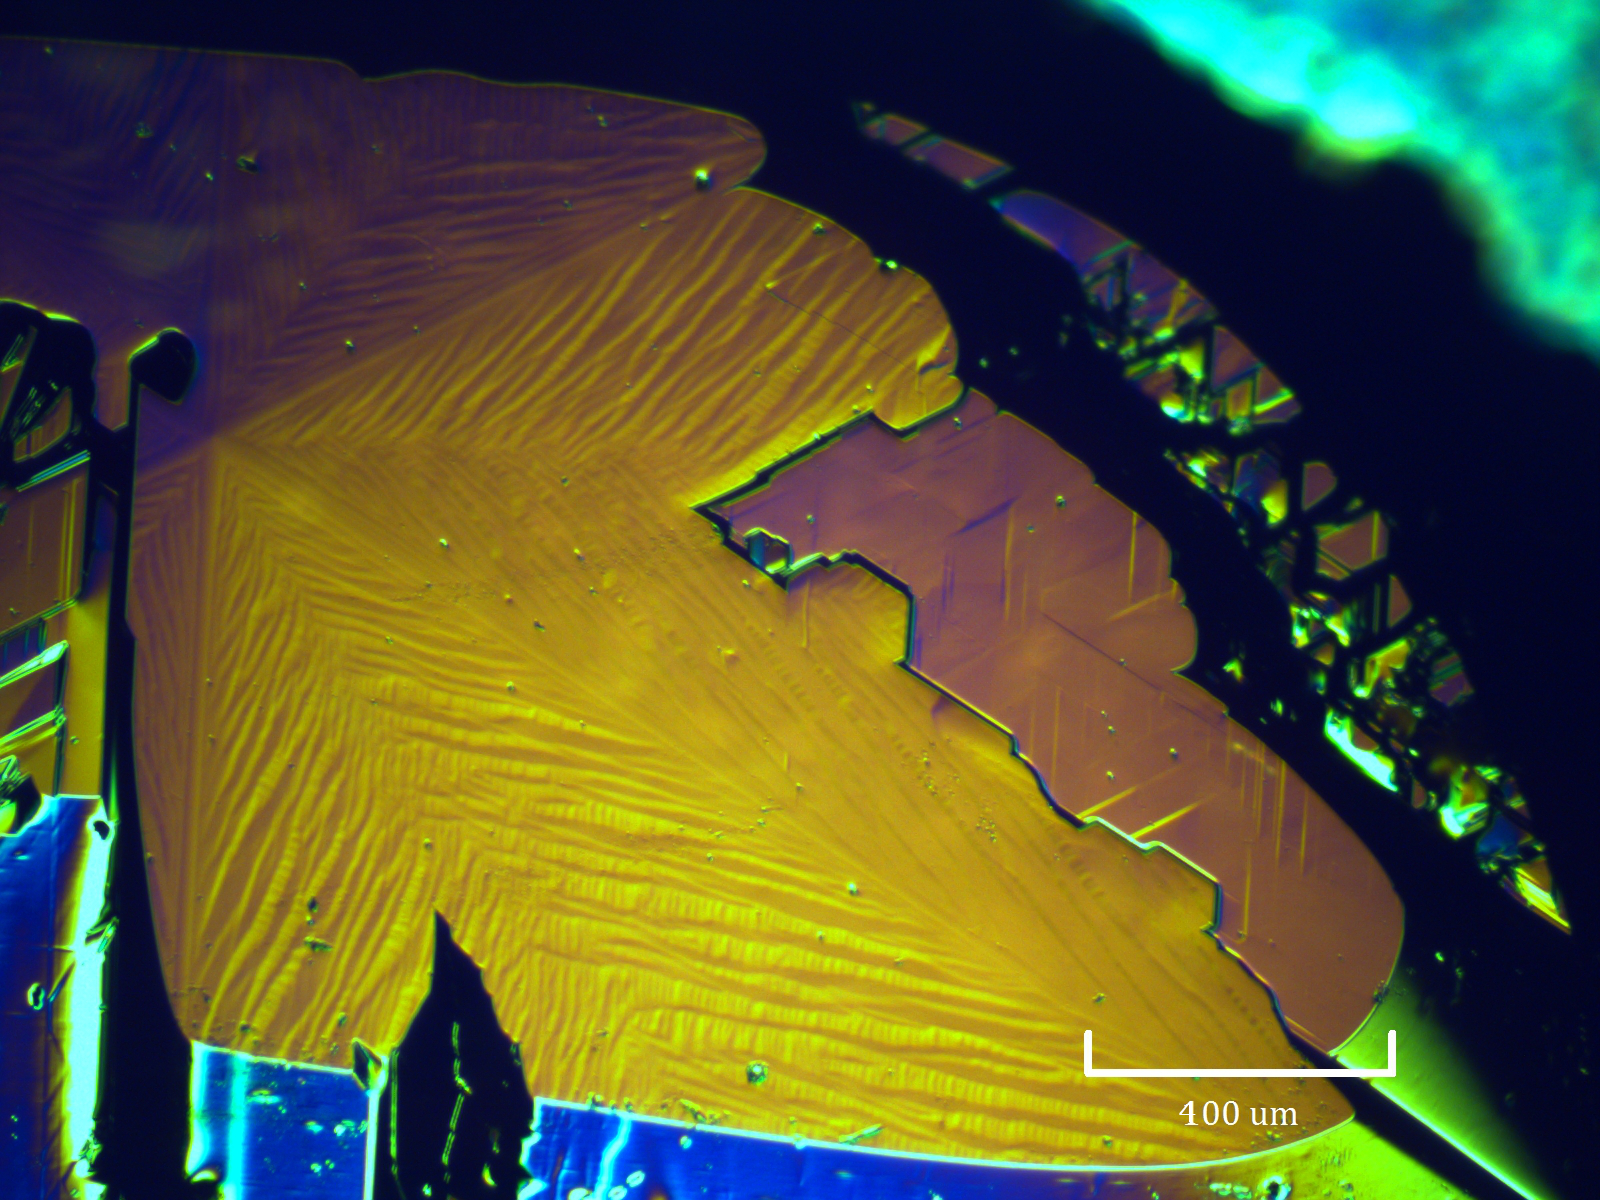
\includegraphics[scale=0.1]{C_seed1.jpg}
  \captionof{figure}{Reflection mode micrograph of the facet of C-face seed \#5.}
  \label{fig:carbon_seed1}
\end{minipage}%
\begin{minipage}{.5\textwidth}
  \centering
  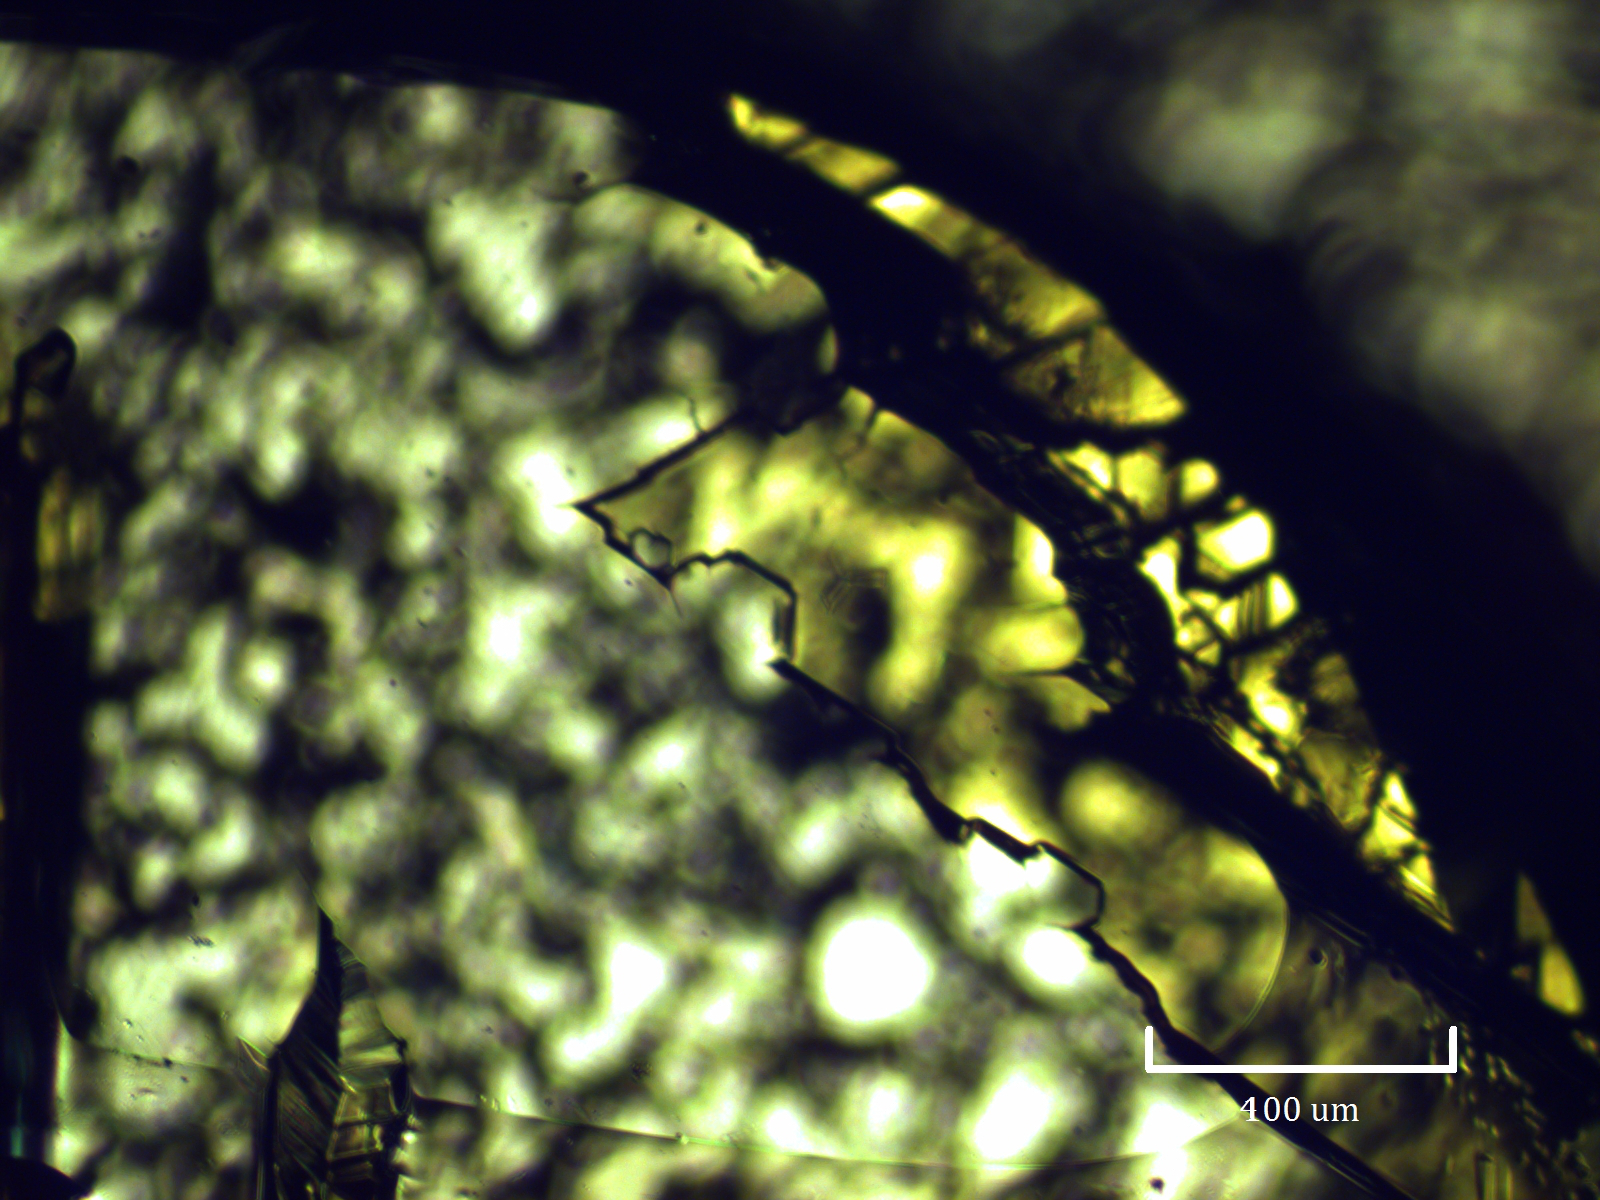
\includegraphics[scale=0.1]{C_seed2.jpg}
  \captionof{figure}{Nomarski transmission mode micrograph of the facet of C-face seed \#5.}
  \label{fig:carbon_seed2}
\end{minipage}
\end{figure}


Table \ref{tab:doped_samples} shows the growth conditions and sample thickness of the grown B-doped samples. The thickness is measured for the doped layer, excluding both the substrate and the undoped seed. The growth mode is the stacking order of the doped and undoped source materials in the crucible, as described in section \ref{sec:growth:fsgp:doping}.


\begin{table}[h]
\caption{Growth conditions of the doped samples are shown in this table. The growth mode describes which samples are grown using direct or indirect doping methods. These methods are described in section \ref{sec:growth:fsgp:doping}. The doping concentration is given for the source material.} 
\label{tab:doped_samples}
\begin{center}
\begin{tabular}{l c c c c r}
  \hline                       
  \hline       
  \vspace{1mm}
   & \small{Temperature [$^\circ$C]} & \small{Time [h:min]} & \small{Thickness [$\mu$m]} & \small{Doping [cm$^{-3}$]} & Mode\\
    \hline
  \#1 & X & X:XX & X & 10$^{18}$&Direct\\ %S1
  \#2 & 1825 & 2:30 & 350 & 10$^{18}$&Direct\\ %S3
  \#3 & 1825 & 3:00 & 360 & 10$^{18}$&Direct\\	%S2
  \#4 & X & X:XX & 440 & 10$^{19}$&Direct\\ %S1
  \#5 & 1825 & 2:30 & 320 & 10$^{19}$&Direct\\ %S2
  \#6 & X & X:XX & X & 10$^{20}$&Direct\\%S1
  \#7 & 1825 & 2:30 & 220 & 10$^{20}$&Direct\\%S2
  \#8 & 1825 & 2:30 & 380 & 10$^{18}$&Indirect\\%S3
%  2 & XXX & X:XX & X & 10$^{20}$&Indirect\\%S2 %BG proper
  \#9 & 1825 & 2:30 & 380 & 10$^{20}$&Indirect\\%S3
  
  \hline  
\end{tabular}
\end{center}
\end{table}
 
Figure \ref{fig:B_doped_micrographs1} shows the surface morphology of an undoped sample (a), doped sample number \#1 (b), doped sample number \#8 (c). The depicted area is chosen to be an area with among the fewest defects possible. It is clearly seen that the undoped sample has a better crystal quality compared to the doped ones. This result was a trend with all grown samples. It should be noted that (b) and (c) show a directly and indirectly doped sample respectively. 

\begin{figure}[h]
\begin{center}
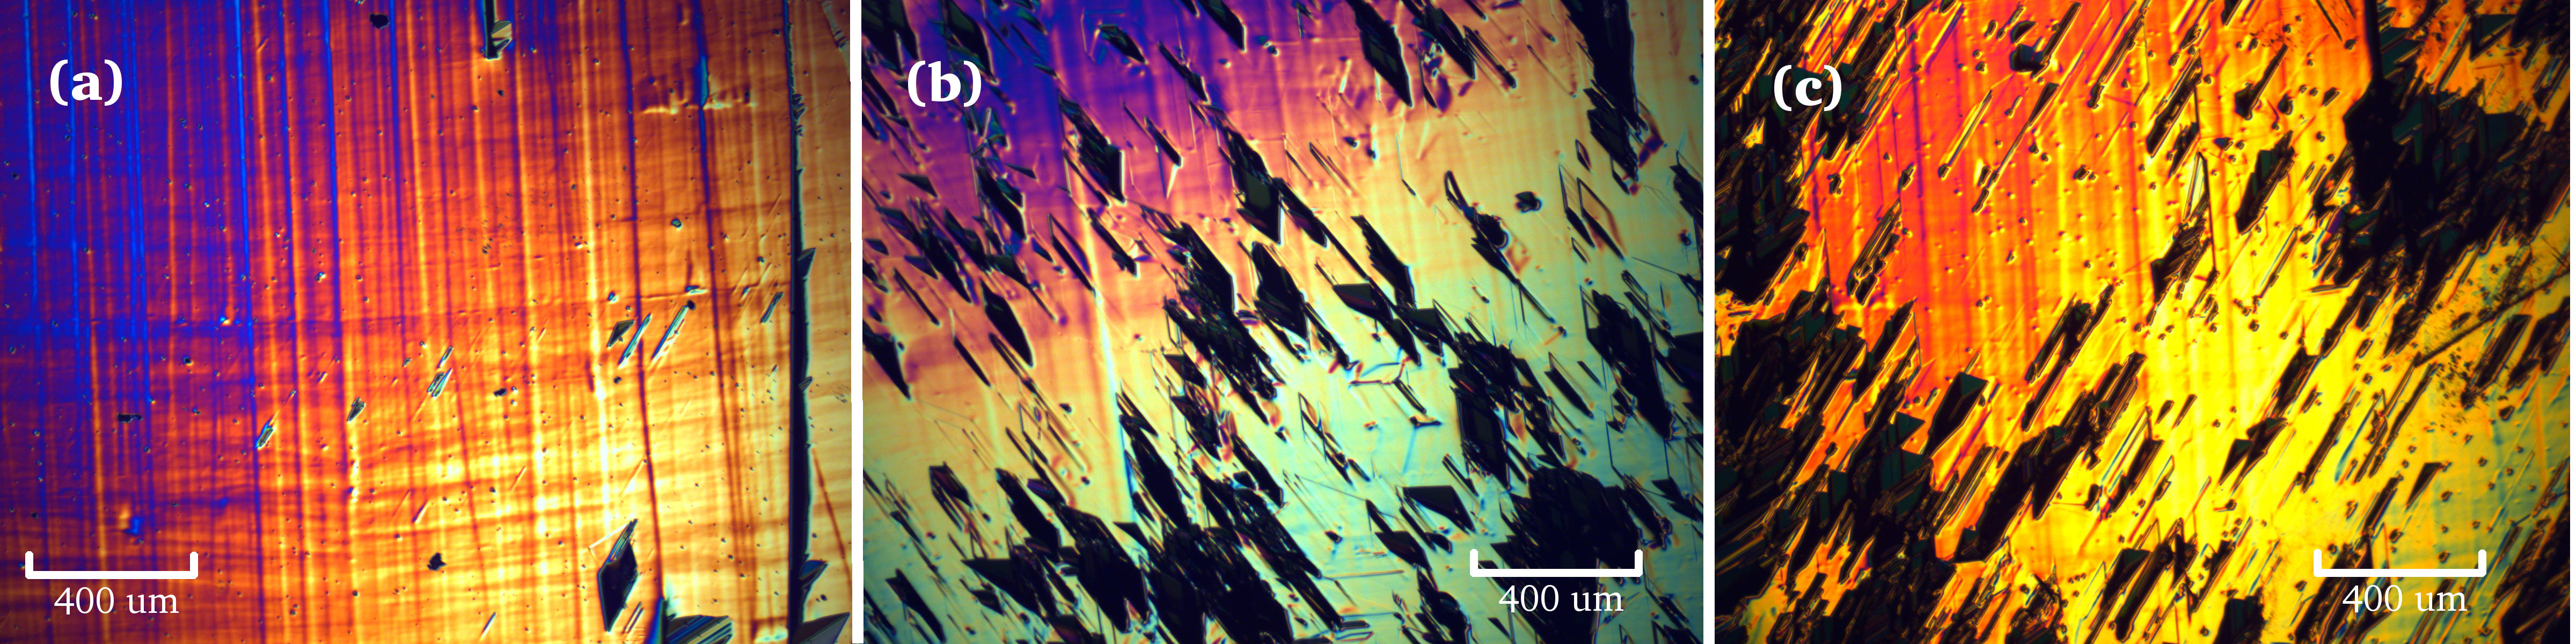
\includegraphics[scale=0.07]{micrographs_doped.jpg}
\caption{Micrographs of an undoped sample (a), doped sample number \#1 (b) and doped sample number \#8 (c).
\label{fig:B_doped_micrographs1}}
\end{center}
\end{figure}

Figure \ref{fig:B_doped_micrographs2} (a)-(c) shows micrographs of samples \#1, \#4 and \#6 respectively. It should be noted that these samples are grown using a source material doped with dopant concentration of 10$^{18}$, 10$^{19}$ and 10$^{20}$ cm$^{-3}$ respectively. From the figures it can be seen that (a) and (b) have a significant density of defects on the surface. Figure (c) shows the smoothest surface, but some defects can still be seen. 

\begin{figure}[h]
\begin{center}
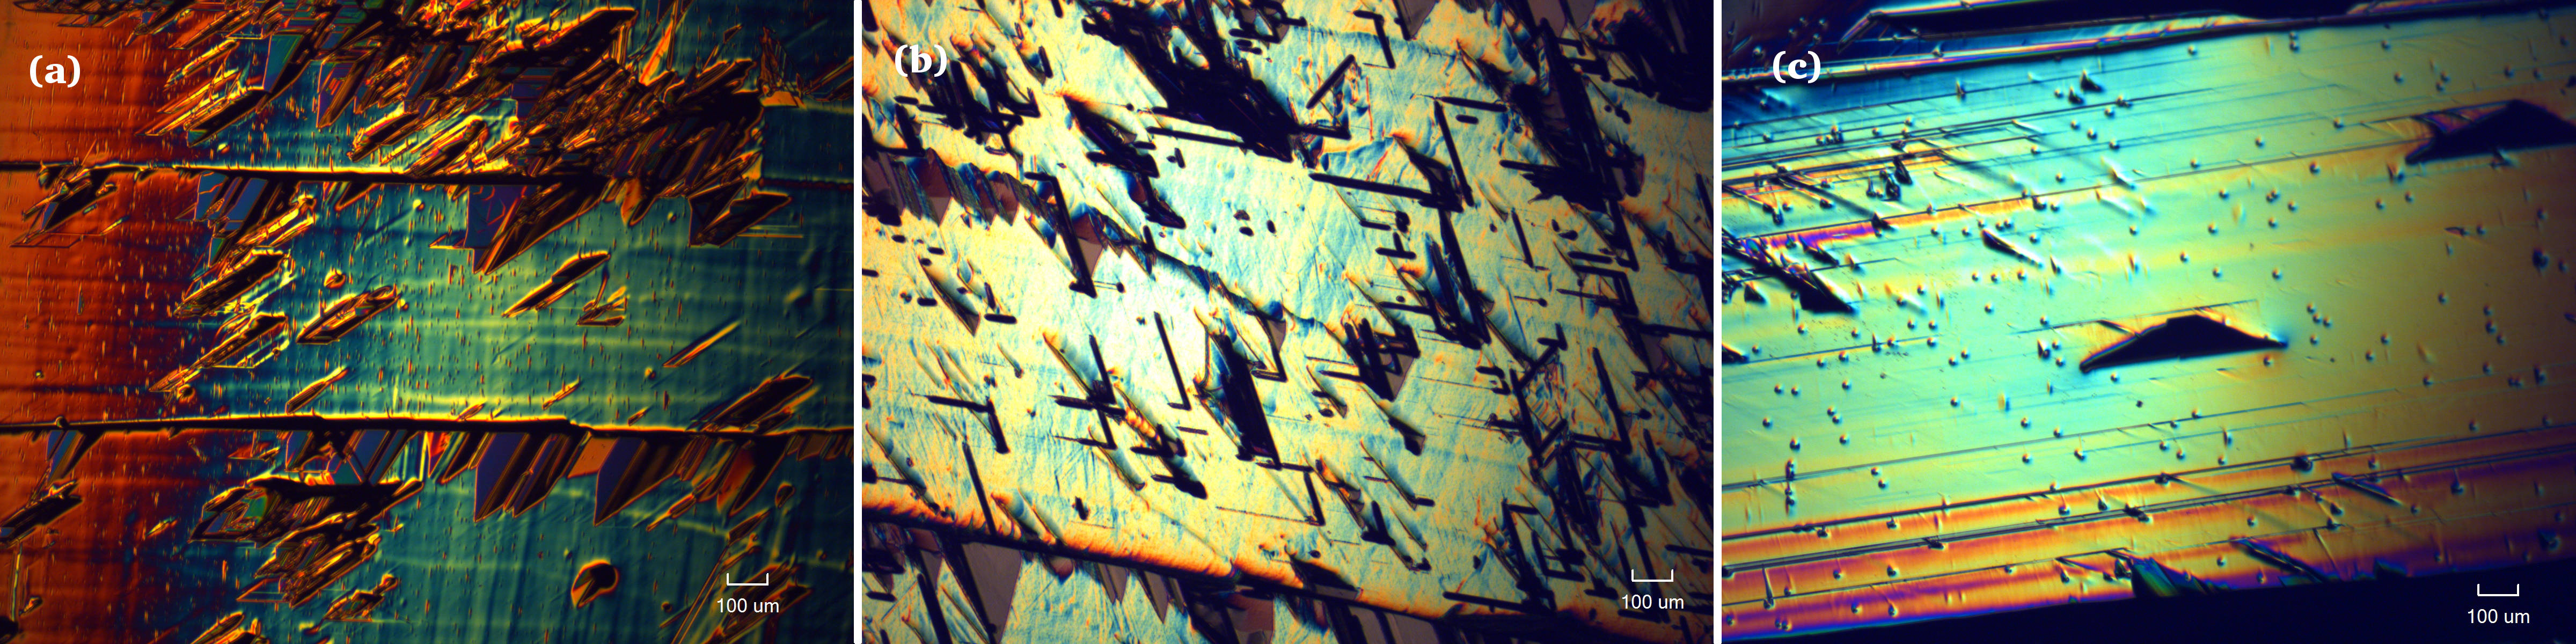
\includegraphics[scale=0.07]{doped_series.jpg}
\caption{Micrographs of doped samples with increasing source doping concentration. Figures (a)-(c) show samples \#1, \#4 and \#6 respectively.
\label{fig:B_doped_micrographs2}}
\end{center}
\end{figure}

Figure \ref{fig:BGe20_micrograph} shows a transmission mode micrograph of sample \#9. It can be seen that there are two different polytypes in the sample. The brighter area in the center is a foreign polytype inclusion. 

\begin{figure}[h]
\begin{center}
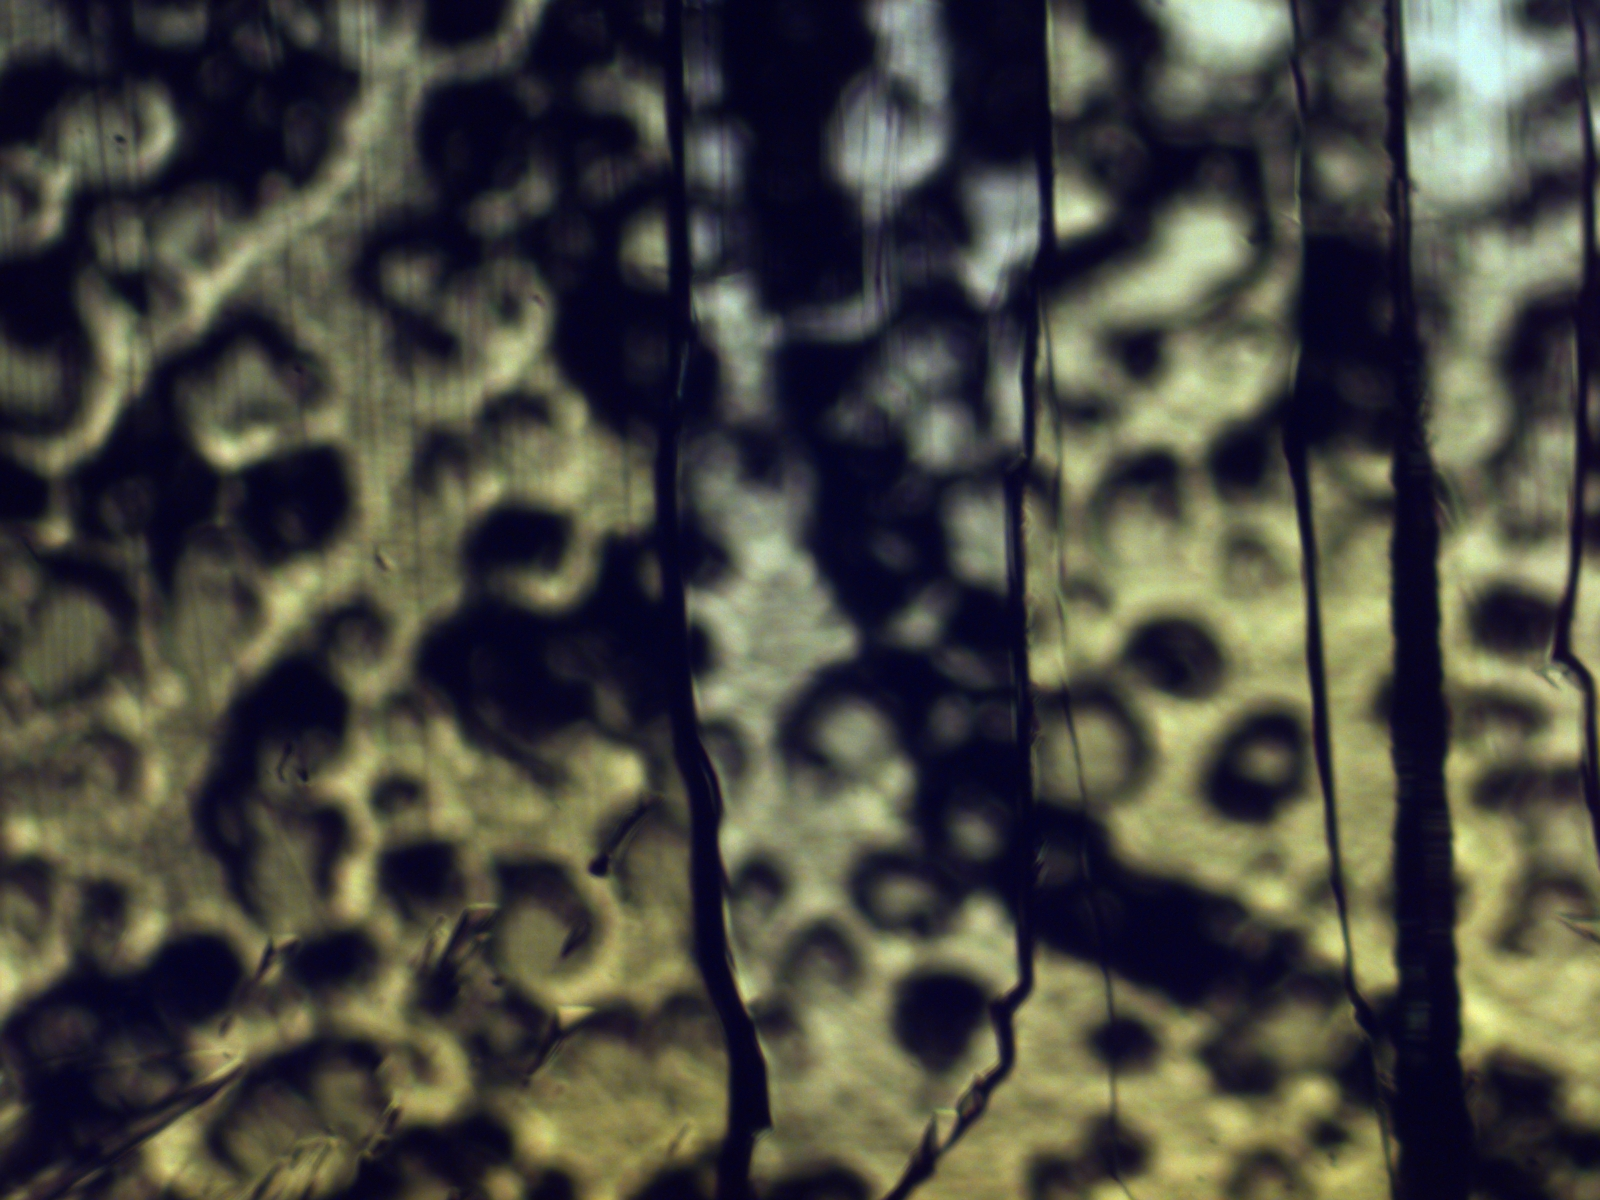
\includegraphics[scale=0.15]{E20_bg4.jpg}
\caption{Transmission mode micrograph of doped sample \#9. The brightness contrast shows a foreign polytype inclusion in the center. 
\label{fig:BGe20_micrograph}}
\end{center}
\end{figure}

Absorption measurements were done on directly doped samples with different source doping concentrations, samples \#1 and \#5. The results of these measurements are shown in figure \ref{fig:abs1}, together with a reference spectrum from an undoped sample (dotted line). In both samples we see the VB to nitrogen transition at around 500 nm. A second feature in the doped sample spectra is the peak at around 700 nm, corresponding to the transition between the boron and nitrogen levels. This cannot be seen in the undoped sample. The doped samples show no evidence for a VB to boron transition, which should be seen at around 1800 nm, as described in chapter \ref{sec:doping_in_3C}. Absorption was also measured for doped samples \#6 and \#7, but neither the band edge nor the boron related peaks was seen in these highly doped samples. 

\begin{figure}[h]
\begin{center}
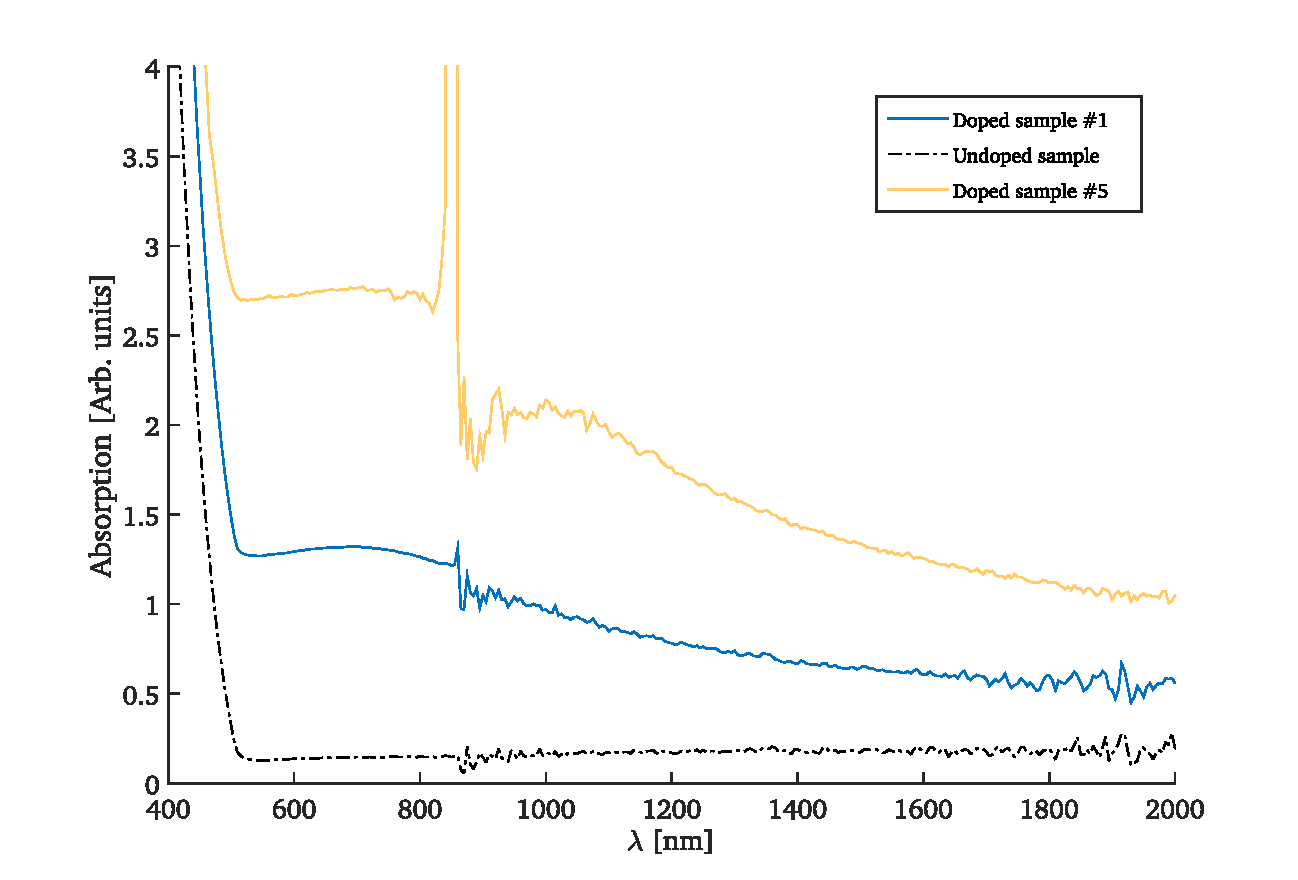
\includegraphics[scale=0.5]{absorption1.pdf}
\caption{Absorption spectrum of undoped sample (dotted line), doped sample \#5 (bright yellow line) and doped sample \#1 (dark blue line). 
\label{fig:abs1}}
\end{center}
\end{figure}

\begin{figure}[h]
\begin{center}
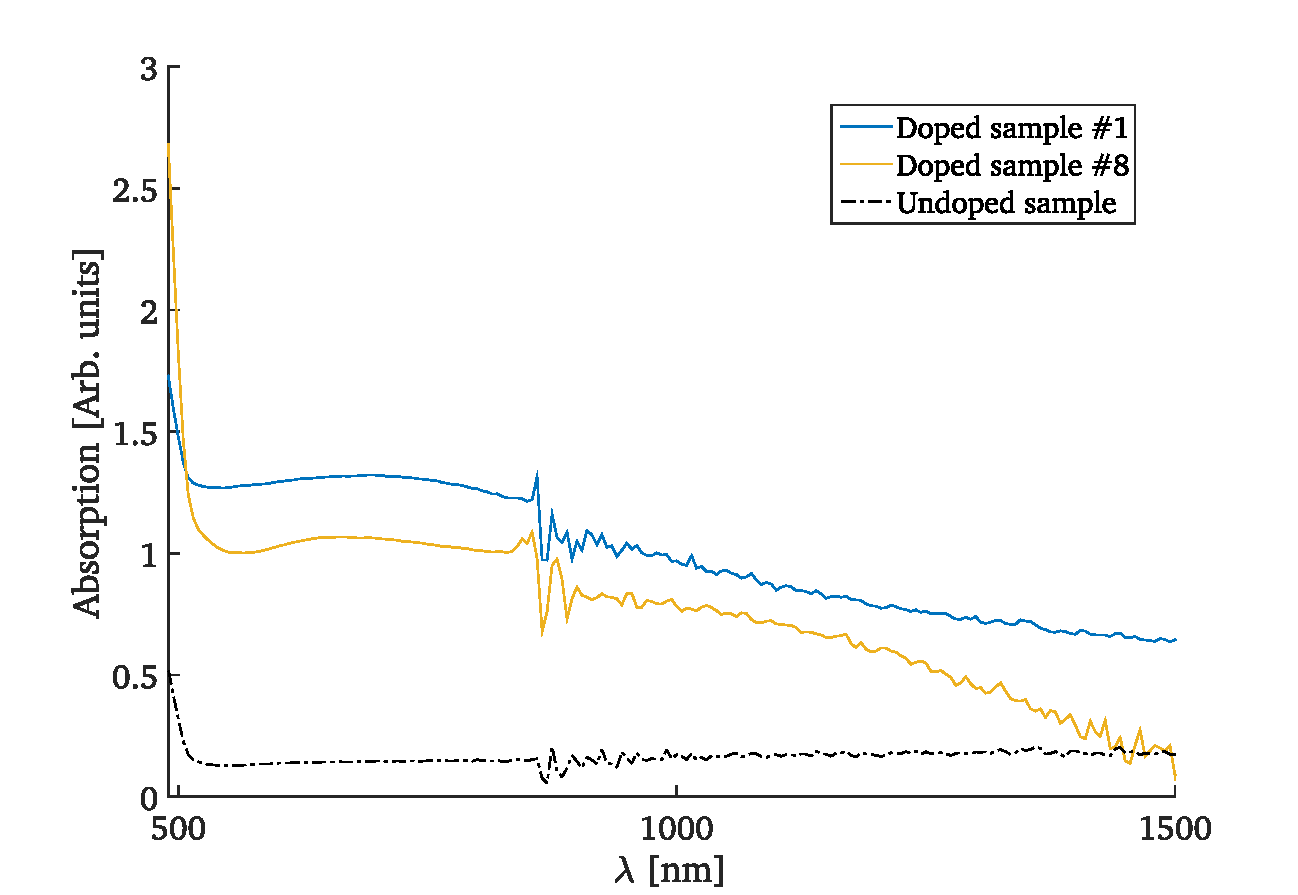
\includegraphics[scale=0.5]{absorption2.pdf}
\caption{Absorption spectrum of doped samples \#8 (bright yellow line) and \#1 (dark blue line), shown together with an undoped sample (dotted line). 
\label{fig:abs2}}
\end{center}
\end{figure}

Figure \ref{fig:abs2} shows the result of absorption measurements on samples \#1 and \#8, together with an undoped sample. It should be noted that \#8 is an indirectly doped sample. It can be seen that both the doped sample spectra show the same trend. The graphs increase up to a point near the 700 nm B-N transition energy, where they level out. This is not visible in the undoped sample. It can further be seen that sample \#8 has its B-N maximum at a slightly shorter wavelength compared to sample \#1. 



LTPL-measurements were done on boron doped samples and on an undoped seed. Figure \ref{fig:pl_spectrum1} shows the resulting spectrum of the undoped seed. Five peaks can clearly be seen in the spectrum, labeled as ZPL and phonon replicas. It should be noted that the ZPL is significantly smaller than the phonon replicas. It can further be seen that several smaller peaks appear on the low energy side of the phonon replicas. These lines originate from exciton complexes.  

\begin{figure}[h]
\begin{center}
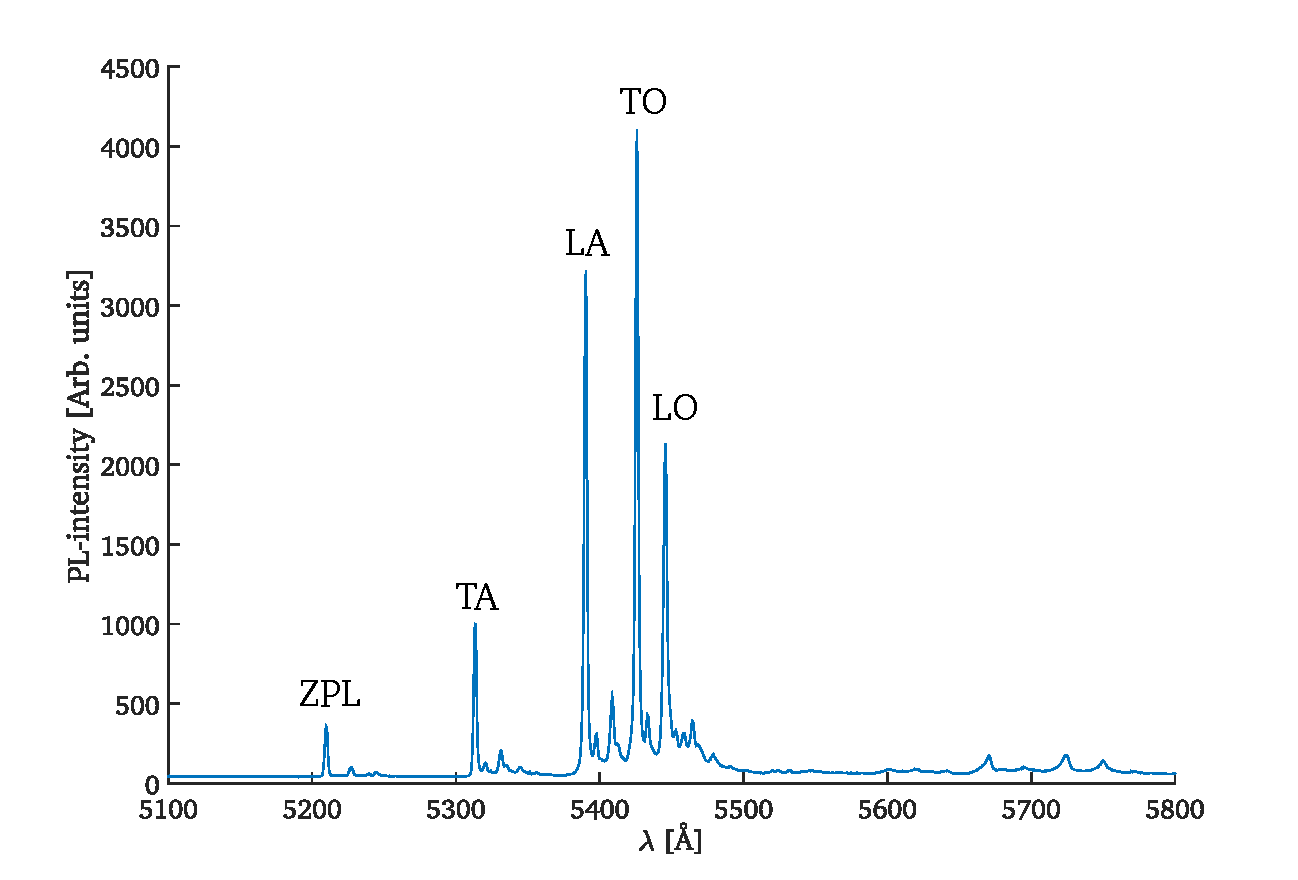
\includegraphics[scale=0.5]{PL_plot1.pdf}
\caption{LTPL spectrum of an undoped seed. The five main peaks are labeled as ZPL and phonon replicas. 
\label{fig:pl_spectrum1}}
\end{center}
\end{figure}

As described in chapter \ref{sec:pl}, the strain in a crystal can be estimated by the fraction between the LA and TO lines. From figure \ref{fig:pl_spectrum1} this is found to be 
\[I_\mathrm{LA}/I_\mathrm{TO} = 0.783.\]
From the TA-line FWHM, the donor concentration can be found. The FWHM is found to be $\Gamma_{TA} = 1.094$ meV, giving a nitrogen concentration of 
\[[N] \approx 10^{16} \, \mathrm{cm^{-3}}.\]

Doped samples \#1, \#4 and \#6 were measured using LTPL. Not one of these samples show any luminescence. Sample \#9 did show luminescence, and the spectrum is shown in figure \ref{fig:pl_spectrum2}. 

<Figure>.


































